\documentclass[11pt,letterpaper]{report}

% --- Paquetes Requeridos ---
\usepackage[utf8]{inputenc}
\usepackage[T1]{fontenc}
\usepackage{lmodern}
\usepackage[letterpaper, margin=2.5cm]{geometry}
\usepackage{amsmath,amssymb}
\usepackage{xcolor}
\usepackage{graphicx}
\usepackage{booktabs}
\usepackage{tabularx}
\usepackage{multirow}
\usepackage{parskip}
\usepackage{microtype}
\usepackage{soul}
\usepackage[hidelinks]{hyperref}

% --- Configuración de Estilo ---
\renewcommand{\familydefault}{\sfdefault}
\setcounter{secnumdepth}{3}

% --- Macro para Fichas de Indicador ---
% Parámetros: {#1 Título}{#2 Nombre}{#3 Objetivo}{#4 Fórmula}
%             {#5 Código}{#6 Resp. gestión}{#7 Resp. carga}{#8 Meta}{#9 Frecuencia}
\newcommand{\fichaIndicador}[9]{
  \noindent
  \begin{tabularx}{\textwidth}{p{0.25\textwidth}XX}
  \toprule
  \textbf{#1} & \multicolumn{2}{c}{\textbf{FICHA DE INDICADOR}} \\
  \midrule
  \textbf{Nombre del indicador} & \textbf{Objetivo del indicador} & \textbf{Fórmula del indicador} \\
  #2 & #3 & #4 \\
  \midrule
  \textbf{Código del indicador} & \textbf{Responsable de gestión} & \textbf{Resp. de carga y reporte} \\
  #5 & #6 & #7 \\
  \midrule
  \textbf{Meta anualizada} & \textbf{Frecuencia de reporte} & \textbf{Fecha de actualización} \\
  #8 & #9 & Por definir \\
  \bottomrule
  \end{tabularx}
  \vspace{1.5em}
}

% --- Datos del Documento ---
\title{\textbf{\large MANUAL DE PROCESOS OPERATIVOS Y DE APOYO}\\[0.5em] \textbf{\Huge CO LOGISTIC SAC}}
\author{\textbf{LOGO COLOGISTIC}}
\date{}

\begin{document}

\maketitle

% --- Control de Versiones ---
\begin{center}
\textbf{\large CONTROL DE VERSIONES}
\end{center}
\begin{tabularx}{\textwidth}{p{0.25\textwidth}p{0.2\textwidth}p{0.2\textwidth}X}
\toprule
\textbf{Aprobado por Acuerdo de} & \textbf{Fecha de Aprobación} & \textbf{Fecha de Vigencia} & \textbf{Notas de la versión} \\
\midrule
Pendiente de aprobación por la Gerencia de Co Logistic SAC & Por definir & Por definir & \begin{itemize} \item Versión 1.0. Documento elaborado a partir de entrevistas al Analista de Inventarios y evidencia documental (guías de remisión, borrador manuscrito de flujo). \item Revisado por el equipo del Proyecto de Fin de Carrera, área de Gestión de Tecnologías de Información (GTI), UPeU. \end{itemize} \\
\bottomrule
\end{tabularx}

\newpage

% --- Índice General ---
\tableofcontents

\newpage

% ==========================================
\chapter{Generalidades}
% ==========================================

\section{Objetivo}
Documentar de manera formal los macroprocesos, procesos y procedimientos que ejecuta Co Logistic SAC como operador logístico (3PL), estableciendo el estado actual (AS-IS) de sus actividades de recepción, almacenamiento, despacho, acondicionamiento de mercadería, arrendamiento de espacios y facturación, con el fin de servir como línea base para la mejora de procesos y la propuesta de automatización mediante tecnologías de información.

\section{Alcance}
El presente manual cubre los macroprocesos operativos (misionales) de \textbf{Gestión de almacén} y \textbf{Arrendamiento de espacios}, así como los procesos de apoyo de \textbf{Facturación} y \textbf{Seguridad y vigilancia}, en tanto se ejecutan en las instalaciones de Co Logistic SAC. Se excluyen del alcance los procesos estratégicos (Gestión de Planeación Estratégica, Gestión de Expansión Estratégica, Gestión Financiera) y los procesos de apoyo de Talento Humano y Mantenimiento, al ser desarrollados por otro equipo dentro del proyecto integrador.

\section{Base Legal}
\begin{enumerate}
  \item \textbf{Resolución de Superintendencia N.° 188-2010/SUNAT y modificatorias:} Regula la emisión de la Guía de Remisión Electrónica (GRE), documento que sustenta el traslado de bienes y constituye el insumo de entrada de los procesos de Recepción y Despacho de mercadería.
  \item \textbf{Resolución de Superintendencia N.° 123-2020/SUNAT:} Establece los requisitos mínimos de la Guía de Remisión Electrónica Remitente, conforme a su Anexo V.
  \item \textbf{Resolución de Superintendencia N.° 000108-2026/SUNAT:} Introduce modificaciones al régimen de guías de remisión electrónicas, vigentes desde el 1 de junio de 2026.
\end{enumerate}

\section{Definiciones}
\begin{itemize}
  \item \textbf{Guía de remisión:} Documento electrónico exigido por la SUNAT para sustentar el traslado físico de bienes entre dos puntos, sin que dicho traslado implique necesariamente una transferencia de propiedad. Es emitida por el remitente (dueño de los bienes) y, cuando aplica transporte público, complementada por una guía de remisión del transportista.
  \item \textbf{Pedido de ingreso:} Documento interno generado por Co Logistic SAC durante el proceso de Recepción, que registra los datos de transporte y de mercadería (código, lote, fecha de vencimiento, pallets, factor, cajas) no contenidos en la guía de remisión del cliente.
  \item \textbf{Pedido de salida (P.S.):} Documento interno generado durante el proceso de Despacho, equivalente al pedido de ingreso, que además incorpora la zona, el stock y el lote/fecha de vencimiento del código solicitado por el cliente.
  \item \textbf{FEFO (First Expired, First Out):} Regla de negocio aplicada en el despacho de mercadería, según la cual se prioriza la salida del lote con la fecha de vencimiento más próxima.
  \item \textbf{Reempaque:} Procedimiento del proceso de Almacenamiento mediante el cual se divide el registro de una paleta cuando su composición física no coincide con lo declarado en la guía de remisión.
  \item \textbf{Unidad comercial:} Atributo configurado a nivel de código de producto que determina si su registro se realiza por caja (aplicando pallet y factor de conversión) o por unidad (sin pallet ni factor), conforme a la naturaleza del producto.
  \item \textbf{Acondicionamiento de mercadería:} Proceso opcional, activado únicamente ante solicitud comercial del cliente, que comprende los servicios de repaletizado y reencajado.
\end{itemize}

\newpage

% ==========================================
\chapter{Disposiciones Complementarias}
% ==========================================

\section{Diagrama General de Procesos}

% --- Tabla SIPOC General: Procesos Misionales / Operativos ---
\subsection*{SIPOC General — Procesos Misionales / Operativos}
\begin{center}
  \small
  \begin{tabularx}{\textwidth}{>{\centering\arraybackslash}X >{\centering\arraybackslash}X >{\centering\arraybackslash}X >{\centering\arraybackslash}X >{\centering\arraybackslash}X}
  \toprule
  \textbf{S} & \textbf{I} & \textbf{P} & \textbf{O} & \textbf{C} \\
  \textbf{Proveedores (del Proceso)} & \textbf{Elementos de entrada} & \textbf{Proceso} & \textbf{Productos (Elementos de Salida)} & \textbf{Clientes (del Proceso)} \\
  \midrule
  \textit{Cliente} & \textit{Guía de remisión} & \textit{Recepción de mercadería} & \textit{Pedido de ingreso aprobado, impreso y engrampado a la guía} & \textit{Almacenamiento} \\
  \midrule
  \textit{Recepción de mercadería} & \textit{Pedido de ingreso aprobado, impreso y engrampado a la guía} & \textit{Almacenamiento} & \textit{Mercadería ubicada y reporte de movimientos actualizado} & \textit{Despacho de mercadería} \\
  \midrule
  \textit{Almacenamiento; Cliente} & \textit{Mercadería ubicada y reporte de movimientos actualizado; nueva guía de remisión de salida} & \textit{Despacho de mercadería} & \textit{Pedido de salida (P.S.) aprobado, impreso y engrampado a la guía} & \textit{Cliente} \\
  \midrule
  \textit{Cliente} & \textit{Solicitud comercial de repaletizado o reencajado} & \textit{Acondicionamiento de mercadería} & \textit{Reporte manual de servicio (código, cantidad, paletas, tarifa)} & \textit{Facturación} \\
  \midrule
  \textit{Cliente; Notario} & \textit{Contrato de arrendamiento} & \textit{Arrendamiento de espacios} & \textit{Espacio entregado en uso} & \textit{Cliente arrendatario} \\
  \bottomrule
  \end{tabularx}
\end{center}


\begin{figure}[h!]
  \centering
  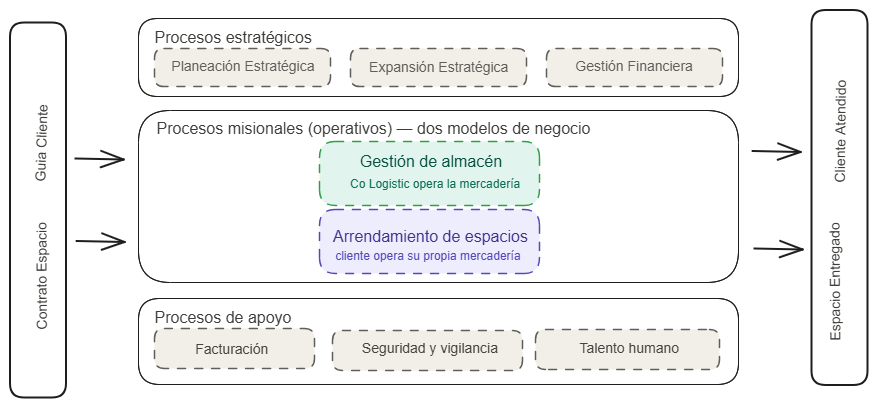
\includegraphics[width=0.95\textwidth]{./imagenes/mapa_operativo_nivel0.png}
  \caption{Mapa de Procesos Nivel 0 — Cadena de valor de Co Logistic SAC (procesos estratégicos, misionales y de apoyo)}
\end{figure}




\vspace{2em}

% --- Tabla SIPOC General: Procesos de Apoyo ---
\subsection*{SIPOC General — Procesos de Apoyo}
\begin{center}
  \small
  \begin{tabularx}{\textwidth}{>{\centering\arraybackslash}X >{\centering\arraybackslash}X >{\centering\arraybackslash}X >{\centering\arraybackslash}X >{\centering\arraybackslash}X}
  \toprule
  \textbf{S} & \textbf{I} & \textbf{P} & \textbf{O} & \textbf{C} \\
  \textbf{Proveedores (del Proceso)} & \textbf{Elementos de entrada} & \textbf{Proceso} & \textbf{Productos (Elementos de Salida)} & \textbf{Clientes (del Proceso)} \\
  \midrule
  \textit{Recepción; Almacenamiento; Despacho; Acondicionamiento} & \textit{Reporte de movimientos; reportes de Acondicionamiento} & \textit{Facturación} & \textit{Factura mensual al cliente} & \textit{Cliente; Contador} \\
  \midrule
  \textit{Cliente; Almacenamiento; Arrendamiento de espacios} & \textit{Acceso de personas, vehículos y mercadería a las instalaciones} & \textit{Seguridad y vigilancia} & \textit{Control de acceso e instalaciones resguardadas} & \textit{Gestión de almacén; Arrendamiento de espacios} \\
  \bottomrule
  \end{tabularx}
\end{center}

\vspace{2em}



\begin{figure}[h!]
  \centering
  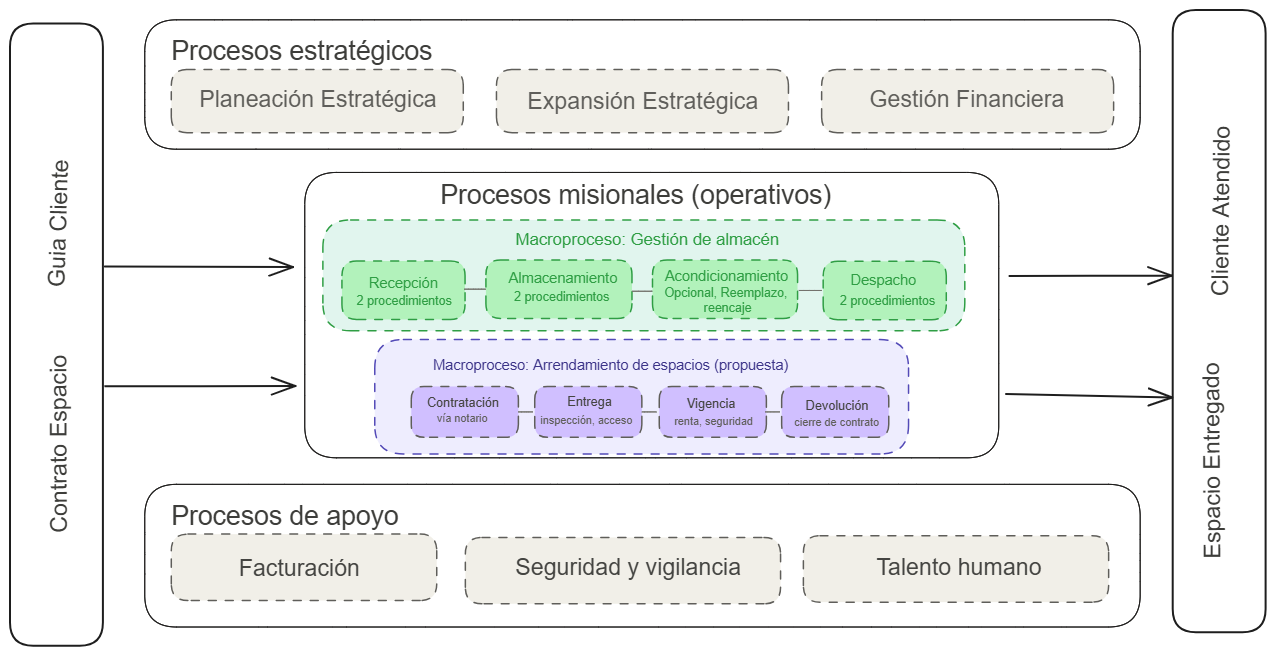
\includegraphics[width=0.95\textwidth]{./imagenes/mapa_operativo_nivel1.png}
  \caption{Mapa de Procesos Nivel 1 — Macroproceso Gestión de almacén}
\end{figure}






\begin{figure}[h!]
  \centering
  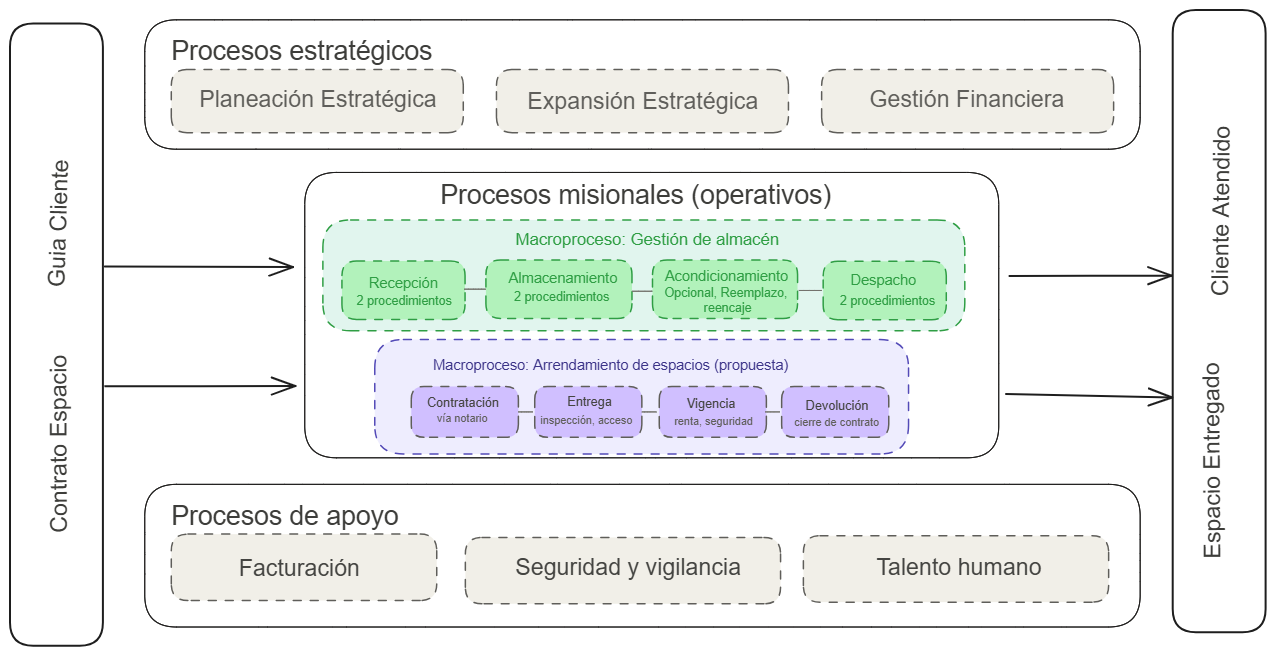
\includegraphics[width=0.95\textwidth]{./imagenes/mapa_operativo_nivel1.png}
  \caption{Mapa de Procesos Nivel 1 — Macroproceso Arrendamiento de espacios}
\end{figure}

\vspace{1.5em}





\noindent\textit{Nota: los procesos estratégicos (Gestión de Planeación Estratégica, Gestión de Expansión Estratégica, Gestión Financiera) se excluyen del presente manual, al ser desarrollados por otro equipo de trabajo dentro del proyecto integrador.}

\vspace{3em}

% --- Tabla Macro Proceso → Proceso → Procedimientos ---
\begin{center}
  \small
  \begin{tabularx}{\textwidth}{p{0.15\textwidth}p{0.18\textwidth}XXp{0.25\textwidth}}
  \toprule
  \multicolumn{2}{c}{\textbf{Macro Proceso}} & \multicolumn{2}{c}{\textbf{Proceso}} & \multirow{2}{*}{\textbf{Procedimientos}} \\
  \cmidrule(r){1-2} \cmidrule(l){3-4}
  \textbf{Título} & \textbf{Líder} & \textbf{Título} & \textbf{Líder} & \\
  \midrule
  \multirow{8}{=}{Gestión de almacén} & \multirow{8}{=}{Gerente de Operaciones} & Recepción de mercadería & Analista de inventarios &
  \begin{itemize} \item Registro de pedido de ingreso \item Verificación y conformidad \end{itemize} \\
  \cmidrule{3-5}
  & & Almacenamiento & Analista de inventarios &
  \begin{itemize} \item Transferencia de ubicación \item Reempaque \end{itemize} \\
  \cmidrule{3-5}
  & & Despacho de mercadería & Analista de inventarios &
  \begin{itemize} \item Registro de pedido de salida \item Verificación y conformidad \end{itemize} \\
  \cmidrule{3-5}
  & & Acondicionamiento de mercadería (opcional) & Auxiliar de almacén &
  \begin{itemize} \item Repaletizado \item Reencajado \end{itemize} \\
  \midrule
  Arrendamiento de espacios & Gerente de Operaciones & Administración de contratos de arrendamiento & Por definir &
  \begin{itemize} \item Contratación (vía notario) \item Entrega \item Vigencia \item Devolución \end{itemize} \\
  \midrule
  Facturación \newline (proceso de apoyo) & Contador & Liquidación mensual & Contador &
  \begin{itemize} \item Liquidación mensual in-out y servicios \end{itemize} \\
  \bottomrule
  \end{tabularx}
\end{center}

\newpage

% ==========================================
\chapter{Procedimientos}
% ==========================================

% ------------------------------------------
\section{Registro de pedido de ingreso}
% ------------------------------------------
\textbf{Macroproceso:} Gestión de almacén \quad\textbar\quad \textbf{Proceso:} Recepción de mercadería \quad\textbar\quad \textbf{Categoría:} Misional / Operativo

\textbf{Líder:} Analista de inventarios

\textbf{Participantes:}
\begin{itemize}
  \item Cliente
  \item Analista de inventarios
\end{itemize}

\textbf{Descripción del Procedimiento:} \\
El procedimiento inicia cuando el cliente envía la guía de remisión (correo electrónico, físico o WhatsApp). Sin este documento no es posible registrar ningún dato en el sistema. El Analista de inventarios registra los datos de transporte (placa, nombre del chofer, brevete, usuario, fecha y hora) y, por cada código de la guía, determina si su unidad comercial es por caja (registrando pallet, factor de conversión y calculando la suma de cajas mediante \texttt{cajas = pallets × factor}) o por unidad (sin pallet ni factor, aplicable a mercadería de merchandising). El procedimiento concluye con la firma del pedido de ingreso por parte del analista, el chofer y el almacén, y su entrega al almacén para la verificación física.

\vspace{1em}
\begin{center}
  \small
  \begin{tabularx}{\textwidth}{>{\raggedright\arraybackslash}p{0.15\textwidth} >{\raggedright\arraybackslash}p{0.18\textwidth} >{\raggedright\arraybackslash}X >{\raggedright\arraybackslash}p{0.18\textwidth} >{\raggedright\arraybackslash}p{0.15\textwidth}}
  \toprule
  \textbf{S} & \textbf{I} & \textbf{P} & \textbf{O} & \textbf{C} \\
  \textbf{Proveedores} & \textbf{Elementos de Entrada} & \textbf{Proceso / Actividades} & \textbf{Elementos de Salida} & \textbf{Clientes} \\
  \midrule
  Cliente & Guía de remisión & 1. Enviar guía de remisión & Guía recibida & Analista de inventarios \\
  \midrule
  Analista de inventarios & Guía recibida & 2. Registrar pedido de ingreso: datos de transporte & Pedido de ingreso con datos de transporte & Analista de inventarios \\
  \midrule
  Analista de inventarios & Pedido de ingreso con datos de transporte & 3. Registrar mercadería según unidad comercial (caja o unidad) & Pedido de ingreso con cantidades y, si aplica, suma de cajas & Analista de inventarios \\
  \midrule
  Analista de inventarios & Pedido de ingreso con cantidades & 4. Firmar pedido de ingreso & Pedido de ingreso firmado & Almacén (Auxiliar / Supervisor) \\
  \bottomrule
  \end{tabularx}
\end{center}
\vspace{1em}

\begin{figure}[h!]
  \centering
  
\includegraphics[width=0.9\textwidth]{./imagenes/Registro de pedido de ingreso.png}
  \caption{Diagrama de Actividades con BPMN - Registro de pedido de ingreso}
\end{figure}

\newpage



% ------------------------------------------
\section{Verificación y conformidad (Recepción)}
% ------------------------------------------
\textbf{Macroproceso:} Gestión de almacén \quad\textbar\quad \textbf{Proceso:} Recepción de mercadería \quad\textbar\quad \textbf{Categoría:} Misional / Operativo

\textbf{Líder:} Supervisor

\textbf{Participantes:}
\begin{itemize}
  \item Auxiliar de almacén
  \item Supervisor
\end{itemize}

\textbf{Descripción del Procedimiento:} \\
El procedimiento inicia cuando el Auxiliar de almacén recibe el pedido de ingreso y verifica físicamente la mercadería contra lo registrado. El Supervisor determina la conformidad: si la mercadería coincide con la guía, aprueba el pedido; si existen observaciones, modifica el pedido en los campos de cantidad, lote, fecha de vencimiento, zona/ubicación, o ejecuta un reempaque cuando la composición física de la paleta no coincide con lo declarado. En ambos casos, el procedimiento concluye con la impresión del pedido de ingreso y su engrampado físico a la guía de remisión del cliente, quedando dicho conjunto documental archivado.

\vspace{1em}
\begin{center}
  \small
  \begin{tabularx}{\textwidth}{>{\raggedright\arraybackslash}p{0.15\textwidth} >{\raggedright\arraybackslash}p{0.18\textwidth} >{\raggedright\arraybackslash}X >{\raggedright\arraybackslash}p{0.18\textwidth} >{\raggedright\arraybackslash}p{0.15\textwidth}}
  \toprule
  \textbf{S} & \textbf{I} & \textbf{P} & \textbf{O} & \textbf{C} \\
  \textbf{Proveedores} & \textbf{Elementos de Entrada} & \textbf{Proceso / Actividades} & \textbf{Elementos de Salida} & \textbf{Clientes} \\
  \midrule
  Analista de inventarios & Pedido de ingreso firmado & 1. Verificar mercadería contra pedido de ingreso & Mercadería constatada físicamente & Supervisor \\
  \midrule
  Auxiliar de almacén & Mercadería constatada físicamente & 2. Determinar conformidad (¿conforme a la guía?) & Decisión: aprobar (conforme) o modificar (con observación) & Supervisor \\
  \midrule
  Supervisor & Decisión: modificar (con observación) & 3. Modificar pedido (cantidad, lote, FV, zona o reempaque) & Pedido corregido & Supervisor \\
  \midrule
  Supervisor & Decisión: aprobar (conforme); o pedido corregido & 4. Imprimir y engrampar pedido de ingreso con la guía de remisión & Pedido de ingreso + guía (archivado) & Almacenamiento \\
  \bottomrule
  \end{tabularx}
\end{center}
\vspace{1em}

\begin{figure}[h!]
  \centering
  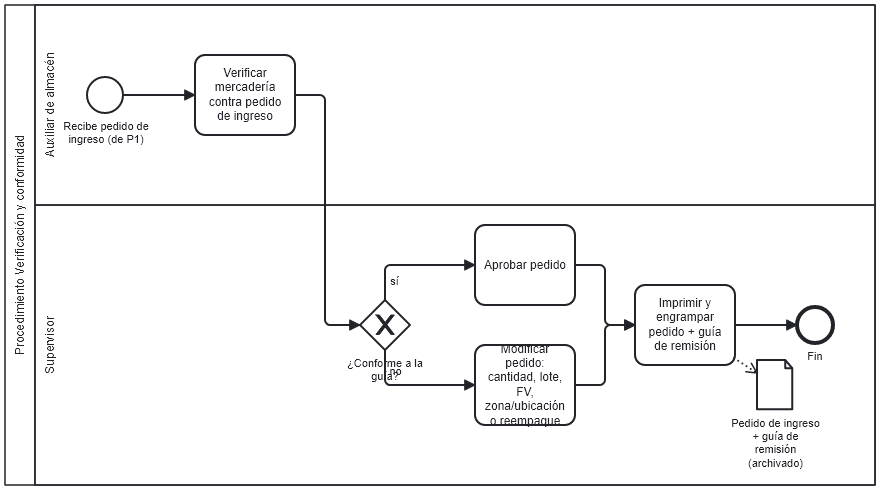
\includegraphics[width=0.9\textwidth]{./imagenes/Recepción de mercadería.png}
  \caption{Diagrama de Actividades con BPMN - Verificación y conformidad (Recepción)}
\end{figure}

\newpage



% ------------------------------------------
\section{Registro de pedido de salida}
% ------------------------------------------
\textbf{Macroproceso:} Gestión de almacén \quad\textbar\quad \textbf{Proceso:} Despacho de mercadería \quad\textbar\quad \textbf{Categoría:} Misional / Operativo

\textbf{Líder:} Analista de inventarios

\textbf{Participantes:}
\begin{itemize}
  \item Cliente
  \item Auxiliar de almacén
  \item Analista de inventarios
\end{itemize}

\textbf{Descripción del Procedimiento:} \\
El procedimiento es estructuralmente similar al de Registro de pedido de ingreso, con los siguientes elementos adicionales propios del despacho. El Auxiliar de almacén realiza el picking, localizando y extrayendo la mercadería según la zona, ubicación y stock disponible del código solicitado (actividad identificada como \textit{picking} en la descripción de funciones del Auxiliar de almacén, conforme a \texttt{Explicacion-puestos-areas-empresa.txt}, y descrita operativamente en \texttt{2-Despacho.txt} sin emplear dicho término técnico). Cuando la guía de remisión del cliente contiene varias líneas (códigos), cada una se registra de manera individual en el sistema. El Analista de inventarios consulta la zona y el stock del código ya recepcionado y, si el código presenta varias fechas de vencimiento, selecciona el lote y la fecha de vencimiento solicitados por el cliente conforme a la regla FEFO (primero en vencer, primero en salir). El registro de la mercadería sigue la misma bifurcación por unidad comercial (caja o unidad) que el proceso de Recepción. El procedimiento concluye con la firma del pedido de salida.

\vspace{1em}
\begin{center}
  \small
  \begin{tabularx}{\textwidth}{>{\raggedright\arraybackslash}p{0.15\textwidth} >{\raggedright\arraybackslash}p{0.18\textwidth} >{\raggedright\arraybackslash}X >{\raggedright\arraybackslash}p{0.18\textwidth} >{\raggedright\arraybackslash}p{0.15\textwidth}}
  \toprule
  \textbf{S} & \textbf{I} & \textbf{P} & \textbf{O} & \textbf{C} \\
  \textbf{Proveedores} & \textbf{Elementos de Entrada} & \textbf{Proceso / Actividades} & \textbf{Elementos de Salida} & \textbf{Clientes} \\
  \midrule
  Cliente & Guía de remisión (1 a 10+ líneas/códigos) & 1. Enviar guía de remisión & Guía recibida & Auxiliar de almacén \\
  \midrule
  Auxiliar de almacén & Guía recibida & 2. Realizar picking: localizar y extraer mercadería según zona, ubicación y stock del código & Mercadería extraída & Analista de inventarios \\
  \midrule
  Analista de inventarios & Mercadería extraída & 3. Registrar pedido de salida (código por código) & Pedido de salida con datos de transporte & Analista de inventarios \\
  \midrule
  Almacenamiento & Pedido de salida con datos de transporte & 4. Consultar zona y stock del código recepcionado & Pedido de salida con zona y stock consultados & Analista de inventarios \\
  \midrule
  Analista de inventarios & Pedido de salida con zona y stock consultados & 5. Seleccionar lote y FV según FEFO (si aplica) & Pedido de salida con lote y FV seleccionados & Analista de inventarios \\
  \midrule
  Analista de inventarios & Pedido de salida con lote y FV seleccionados & 6. Registrar mercadería según unidad comercial (caja o unidad) & Pedido de salida con cantidades & Analista de inventarios \\
  \midrule
  Analista de inventarios & Pedido de salida con cantidades & 7. Firmar pedido de salida & Pedido de salida firmado & Almacén (Auxiliar / Supervisor) \\
  \bottomrule
  \end{tabularx}
\end{center}
\vspace{1em}

\begin{figure}[h!]
  \centering
  
\includegraphics[width=0.9\textwidth]{./imagenes/Despacho de mercadería.png}
  \caption{Diagrama de Actividades con BPMN - Registro de pedido de salida}
\end{figure}

\newpage

% ------------------------------------------
\section{Verificación y conformidad (Despacho)}
% ------------------------------------------
\textbf{Macroproceso:} Gestión de almacén \quad\textbar\quad \textbf{Proceso:} Despacho de mercadería \quad\textbar\quad \textbf{Categoría:} Misional / Operativo

\textbf{Líder:} Supervisor

\textbf{Participantes:}
\begin{itemize}
  \item Auxiliar de almacén
  \item Supervisor
\end{itemize}

\textbf{Descripción del Procedimiento:} \\
Procedimiento idéntico en estructura a la Verificación y conformidad de Recepción, aplicado al pedido de salida (P.S.). El Auxiliar de almacén verifica la mercadería contra el pedido de salida; el Supervisor aprueba o, ante observaciones, modifica el pedido (cantidad, lote, fecha de vencimiento, zona/ubicación o reempaque). El procedimiento concluye con la impresión del pedido de salida y su engrampado a la guía de remisión, quedando el conjunto documental archivado.

\vspace{1em}
\begin{center}
  \small
  \begin{tabularx}{\textwidth}{>{\raggedright\arraybackslash}p{0.15\textwidth} >{\raggedright\arraybackslash}p{0.18\textwidth} >{\raggedright\arraybackslash}X >{\raggedright\arraybackslash}p{0.18\textwidth} >{\raggedright\arraybackslash}p{0.15\textwidth}}
  \toprule
  \textbf{S} & \textbf{I} & \textbf{P} & \textbf{O} & \textbf{C} \\
  \textbf{Proveedores} & \textbf{Elementos de Entrada} & \textbf{Proceso / Actividades} & \textbf{Elementos de Salida} & \textbf{Clientes} \\
  \midrule
  Analista de inventarios & Pedido de salida firmado & 1. Verificar mercadería contra pedido de salida & Mercadería constatada físicamente & Supervisor \\
  \midrule
  Auxiliar de almacén & Mercadería constatada físicamente & 2. Determinar conformidad (¿conforme a la guía?) & Decisión: aprobar (conforme) o modificar (con observación) & Supervisor \\
  \midrule
  Supervisor & Decisión: modificar (con observación) & 3. Modificar pedido (cantidad, lote, FV, zona o reempaque) & Pedido corregido & Supervisor \\
  \midrule
  Supervisor & Decisión: aprobar (conforme); o pedido corregido & 4. Imprimir y engrampar P.S. con la guía de remisión & Pedido de salida + guía (archivado) & Cliente \\
  \bottomrule
  \end{tabularx}
\end{center}
\vspace{1em}

\begin{figure}[h!]
  \centering
  
\includegraphics[width=0.9\textwidth]{./imagenes/Verificación y conformidad.png}
  \caption{Diagrama de Actividades con BPMN - Verificación y conformidad (Despacho)}
\end{figure}

\newpage




% ------------------------------------------
\section{Transferencia de ubicación}
% ------------------------------------------
\textbf{Macroproceso:} Gestión de almacén \quad\textbar\quad \textbf{Proceso:} Almacenamiento \quad\textbar\quad \textbf{Categoría:} Misional / Operativo

\textbf{Líder:} Analista de inventarios

\textbf{Participantes:}
\begin{itemize}
  \item Analista de inventarios
\end{itemize}

\textbf{Descripción del Procedimiento:} \\
Procedimiento de sistema que permite mover un código de una ubicación origen a una ubicación destino dentro del almacén. El Analista de inventarios ingresa el código a transferir, y el sistema muestra las fechas de vencimiento disponibles para dicho código. El analista decide si transfiere la totalidad de las fechas registradas o únicamente una fecha de vencimiento específica, indica la ubicación de origen y destino, y ejecuta la transferencia. El movimiento queda reflejado en el reporte de movimientos.

\vspace{1em}
\begin{center}
  \small
  \begin{tabularx}{\textwidth}{>{\raggedright\arraybackslash}p{0.15\textwidth} >{\raggedright\arraybackslash}p{0.18\textwidth} >{\raggedright\arraybackslash}X >{\raggedright\arraybackslash}p{0.18\textwidth} >{\raggedright\arraybackslash}p{0.15\textwidth}}
  \toprule
  \textbf{S} & \textbf{I} & \textbf{P} & \textbf{O} & \textbf{C} \\
  \textbf{Proveedores} & \textbf{Elementos de Entrada} & \textbf{Proceso / Actividades} & \textbf{Elementos de Salida} & \textbf{Clientes} \\
  \midrule
  Recepción de mercadería & Código previamente recepcionado & 1. Ingresar código a transferir & Código identificado & Analista de inventarios \\
  \midrule
  Analista de inventarios & Código identificado & 2. Consultar fechas de vencimiento disponibles & Lista de fechas disponibles & Analista de inventarios \\
  \midrule
  Analista de inventarios & Lista de fechas disponibles & 3. Seleccionar todas las fechas o una fecha específica & Alcance de la transferencia definido & Analista de inventarios \\
  \midrule
  Analista de inventarios & Alcance de la transferencia definido; ubicación origen y destino & 4. Ejecutar transferencia & Reporte de movimientos actualizado & Despacho de mercadería \\
  \bottomrule
  \end{tabularx}
\end{center}
\vspace{1em}

\begin{figure}[h!]
  \centering
  
\includegraphics[width=0.9\textwidth]{./imagenes/Transferencia ubicación.png}
  \caption{Diagrama de Actividades con BPMN - Transferencia de ubicación}
\end{figure}

\newpage

% ------------------------------------------
\section{Reempaque}
% ------------------------------------------
\textbf{Macroproceso:} Gestión de almacén \quad\textbar\quad \textbf{Proceso:} Almacenamiento \quad\textbar\quad \textbf{Categoría:} Misional / Operativo

\textbf{Líder:} Analista de inventarios

\textbf{Participantes:}
\begin{itemize}
  \item Auxiliar de almacén
  \item Analista de inventarios
\end{itemize}

\textbf{Descripción del Procedimiento:} \\
Procedimiento aplicado cuando la composición física de una paleta no coincide con lo declarado en la guía de remisión (por ejemplo, una paleta declarada como 50 unidades que físicamente llega dividida en dos paletas de 20 y 30). El Auxiliar de almacén constata las paletas tal como llegaron, sin unirlas. El Analista de inventarios selecciona la paleta a reempacar, registra la fecha de vencimiento correspondiente y ejecuta el reempaque, dividiendo el registro en las cantidades correspondientes. El resultado queda reflejado en el reporte de movimientos.

\vspace{1em}
\begin{center}
  \small
  \begin{tabularx}{\textwidth}{>{\raggedright\arraybackslash}p{0.15\textwidth} >{\raggedright\arraybackslash}p{0.18\textwidth} >{\raggedright\arraybackslash}X >{\raggedright\arraybackslash}p{0.18\textwidth} >{\raggedright\arraybackslash}p{0.15\textwidth}}
  \toprule
  \textbf{S} & \textbf{I} & \textbf{P} & \textbf{O} & \textbf{C} \\
  \textbf{Proveedores} & \textbf{Elementos de Entrada} & \textbf{Proceso / Actividades} & \textbf{Elementos de Salida} & \textbf{Clientes} \\
  \midrule
  Recepción de mercadería & Paleta física no coincidente con la guía & 1. Constatar paletas tal como llegaron (sin unirlas) & Paletas constatadas & Analista de inventarios \\
  \midrule
  Auxiliar de almacén & Paletas constatadas & 2. Seleccionar la paleta a reempacar & Paleta seleccionada & Analista de inventarios \\
  \midrule
  Analista de inventarios & Paleta seleccionada & 3. Colocar fecha de vencimiento & Fecha de vencimiento registrada & Analista de inventarios \\
  \midrule
  Analista de inventarios & Fecha de vencimiento registrada & 4. Ejecutar reempaque (dividir paleta en cantidades) & Reporte de movimientos actualizado & Despacho de mercadería \\
  \bottomrule
  \end{tabularx}
\end{center}
\vspace{1em}

\begin{figure}[h!]
  \centering
  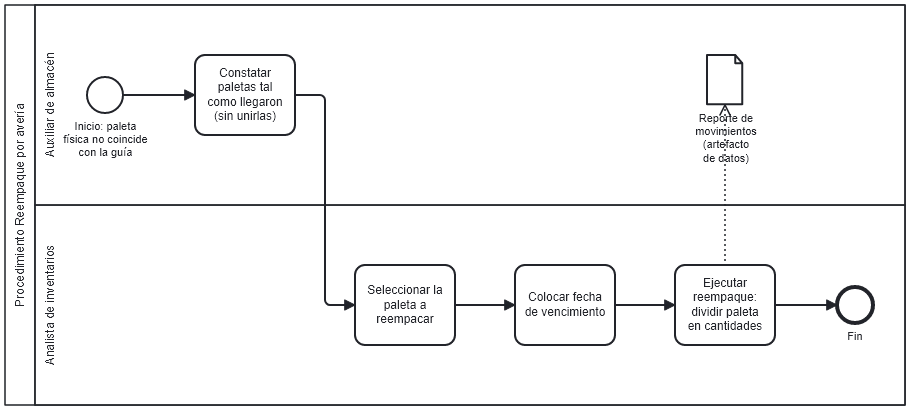
\includegraphics[width=0.9\textwidth]{./imagenes/Reempaque.png}
  \caption{Diagrama de Actividades con BPMN - Reempaque}
\end{figure}

\newpage

% ------------------------------------------
\section{Repaletizado}
% ------------------------------------------
\textbf{Macroproceso:} Gestión de almacén \quad\textbar\quad \textbf{Proceso:} Acondicionamiento de mercadería (opcional) \quad\textbar\quad \textbf{Categoría:} Misional / Operativo

\textbf{Líder:} Auxiliar de almacén

\textbf{Participantes:}
\begin{itemize}
  \item Cliente
  \item Auxiliar de almacén
\end{itemize}

\textbf{Descripción del Procedimiento:} \\
Servicio opcional solicitado comercialmente por el cliente, mediante el cual la mercadería se traslada, caja por caja, desde la paleta en que se encuentra hacia una paleta estándar de exportación, fumigada o certificada, provista en algunos casos por el propio cliente. El procedimiento es enteramente físico, sin soporte en el sistema de información. Concluye con la elaboración manual de un reporte que detalla código, descripción, cantidad, número de paletas y tarifa, el cual constituye el insumo de entrada del proceso de Facturación.

\vspace{1em}
\begin{center}
  \small
  \begin{tabularx}{\textwidth}{>{\raggedright\arraybackslash}p{0.15\textwidth} >{\raggedright\arraybackslash}p{0.18\textwidth} >{\raggedright\arraybackslash}X >{\raggedright\arraybackslash}p{0.18\textwidth} >{\raggedright\arraybackslash}p{0.15\textwidth}}
  \toprule
  \textbf{S} & \textbf{I} & \textbf{P} & \textbf{O} & \textbf{C} \\
  \textbf{Proveedores} & \textbf{Elementos de Entrada} & \textbf{Proceso / Actividades} & \textbf{Elementos de Salida} & \textbf{Clientes} \\
  \midrule
  Cliente & Solicitud de repaletizado por código & 1. Solicitar repaletizado por codigo & Solicitud registrada & Auxiliar de almacén \\
  \midrule
  Cliente & Solicitud registrada & 2. Proveer paleta destino (estándar de exportación, fumigada o certificada, si aplica) & Solicitud registrada; paleta destino disponible & Auxiliar de almacén \\
  \midrule
  Almacenamiento & Solicitud registrada; paleta destino disponible; mercadería en paleta de origen & 3. Trasladar mercadería caja por caja a la nueva paleta & Mercadería repaletizada & Auxiliar de almacén \\
  \midrule
  Auxiliar de almacén & Mercadería repaletizada & 4. Elaborar reporte manual (código, descripción, cantidad, paletas, tarifa) & Reporte manual de repaletizado & Facturación \\
  \bottomrule
  \end{tabularx}
\end{center}
\vspace{1em}

\begin{figure}[h!]
  \centering
  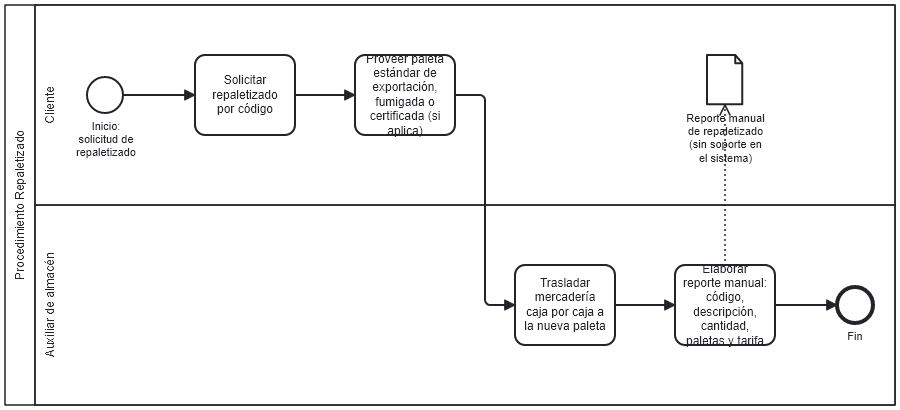
\includegraphics[width=0.9\textwidth]{./imagenes/Repaletizado.png}
  \caption{Diagrama de Actividades con BPMN - Repaletizado}
\end{figure}

\newpage

% ------------------------------------------
\section{Reencajado}
% ------------------------------------------
\textbf{Macroproceso:} Gestión de almacén \quad\textbar\quad \textbf{Proceso:} Acondicionamiento de mercadería (opcional) \quad\textbar\quad \textbf{Categoría:} Misional / Operativo

\textbf{Líder:} Auxiliar de almacén

\textbf{Participantes:}
\begin{itemize}
  \item Cliente
  \item Auxiliar de almacén
\end{itemize}

\textbf{Descripción del Procedimiento:} \\
Servicio opcional solicitado comercialmente por el cliente, similar en su estructura al Repaletizado, mediante el cual la mercadería se traslada de su caja original a una nueva caja indicada por el cliente. El Auxiliar de almacén ejecuta el traslado de forma física y elabora un reporte manual con código, descripción, cantidad y tarifa, el cual constituye insumo de entrada del proceso de Facturación.

\vspace{1em}
\begin{center}
  \small
  \begin{tabularx}{\textwidth}{>{\raggedright\arraybackslash}p{0.15\textwidth} >{\raggedright\arraybackslash}p{0.18\textwidth} >{\raggedright\arraybackslash}X >{\raggedright\arraybackslash}p{0.18\textwidth} >{\raggedright\arraybackslash}p{0.15\textwidth}}
  \toprule
  \textbf{S} & \textbf{I} & \textbf{P} & \textbf{O} & \textbf{C} \\
  \textbf{Proveedores} & \textbf{Elementos de Entrada} & \textbf{Proceso / Actividades} & \textbf{Elementos de Salida} & \textbf{Clientes} \\
  \midrule
  Cliente & Solicitud de reencajado por código & 1. Solicitar reencajado por codigo & Solicitud registrada & Auxiliar de almacén \\
  \midrule
  Cliente & Solicitud registrada & 2. Indicar caja destino & Solicitud registrada; caja destino disponible & Auxiliar de almacén \\
  \midrule
  Almacenamiento & Solicitud registrada; caja destino disponible; mercadería en caja original & 3. Trasladar mercadería a la nueva caja & Mercadería reencajada & Auxiliar de almacén \\
  \midrule
  Auxiliar de almacén & Mercadería reencajada & 4. Elaborar reporte manual (código, descripción, cantidad, tarifa) & Reporte manual de reencajado & Facturación \\
  \bottomrule
  \end{tabularx}
\end{center}
\vspace{1em}

\begin{figure}[h!]
  \centering
  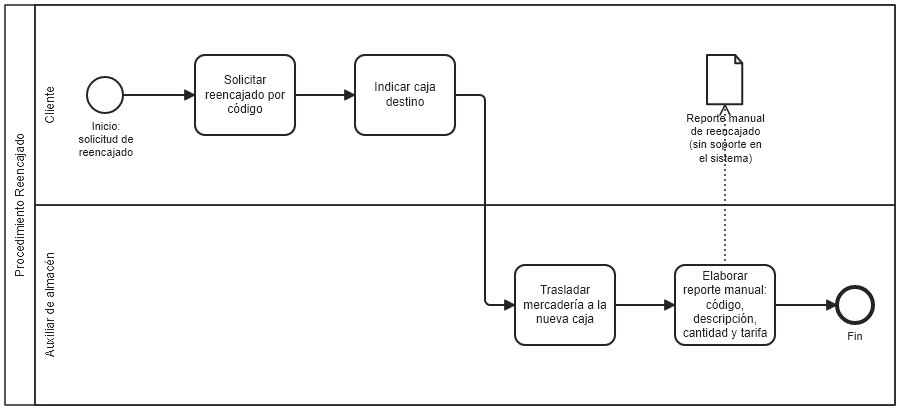
\includegraphics[width=0.9\textwidth]{./imagenes/Reencajado.png}
  \caption{Diagrama de Actividades con BPMN - Reencajado}
\end{figure}

\newpage

% ------------------------------------------
\section{Liquidación mensual in-out y servicios (Facturación)}
% ------------------------------------------
\textbf{Macroproceso:} Procesos de apoyo \quad\textbar\quad \textbf{Proceso:} Facturación \quad\textbar\quad \textbf{Categoría:} Apoyo

\textbf{Líder:} Contador

\textbf{Participantes:}
\begin{itemize}
  \item Analista de inventarios
  \item Contador
\end{itemize}

\textbf{Descripción del Procedimiento:} \\
Proceso de apoyo, desacoplado del flujo operativo de despacho, ejecutado al cierre de cada mes. El Analista de inventarios filtra el reporte de movimientos por tipo de producto y por mes, incorpora los reportes manuales de Acondicionamiento (repaletizado y reencajado) y exporta la información consolidada a una hoja de cálculo en Excel, la cual remite al Contador. El Contador aplica la tarifa correspondiente según el tipo de mercadería (por paleta o por metro cuadrado), prorratea el monto a cobrar conforme a la fecha de corte (días transcurridos sobre 30), y emite la factura correspondiente al cliente. El procedimiento se ejecuta en su totalidad de manera manual, sin soporte específico en el sistema de información.

\vspace{1em}
\begin{center}
  \small
  \begin{tabularx}{\textwidth}{>{\raggedright\arraybackslash}p{0.15\textwidth} >{\raggedright\arraybackslash}p{0.18\textwidth} >{\raggedright\arraybackslash}X >{\raggedright\arraybackslash}p{0.18\textwidth} >{\raggedright\arraybackslash}p{0.15\textwidth}}
  \toprule
  \textbf{S} & \textbf{I} & \textbf{P} & \textbf{O} & \textbf{C} \\
  \textbf{Proveedores} & \textbf{Elementos de Entrada} & \textbf{Proceso / Actividades} & \textbf{Elementos de Salida} & \textbf{Clientes} \\
  \midrule
  Recepción; Almacenamiento; Despacho & Reporte de movimientos del mes & 1. Filtrar reporte de movimientos por tipo y mes & Reporte filtrado & Analista de inventarios \\
  \midrule
  Acondicionamiento de mercadería & Reporte filtrado; reportes de repaletizado y reencajado & 2. Incluir reportes de Acondicionamiento & Reporte consolidado & Analista de inventarios \\
  \midrule
  Analista de inventarios & Reporte consolidado & 3. Exportar reporte a Excel y enviar al contador & Excel enviado & Contador \\
  \midrule
  Contador & Excel enviado; tipo de tarifa (paleta o m²) & 4. Aplicar tarifa y prorratear por fecha de corte & Monto a cobrar calculado & Contador \\
  \midrule
  Contador & Monto a cobrar calculado & 5. Emitir factura al cliente & Factura mensual & Cliente \\
  \bottomrule
  \end{tabularx}
\end{center}
\vspace{1em}

\begin{figure}[h!]
  \centering
  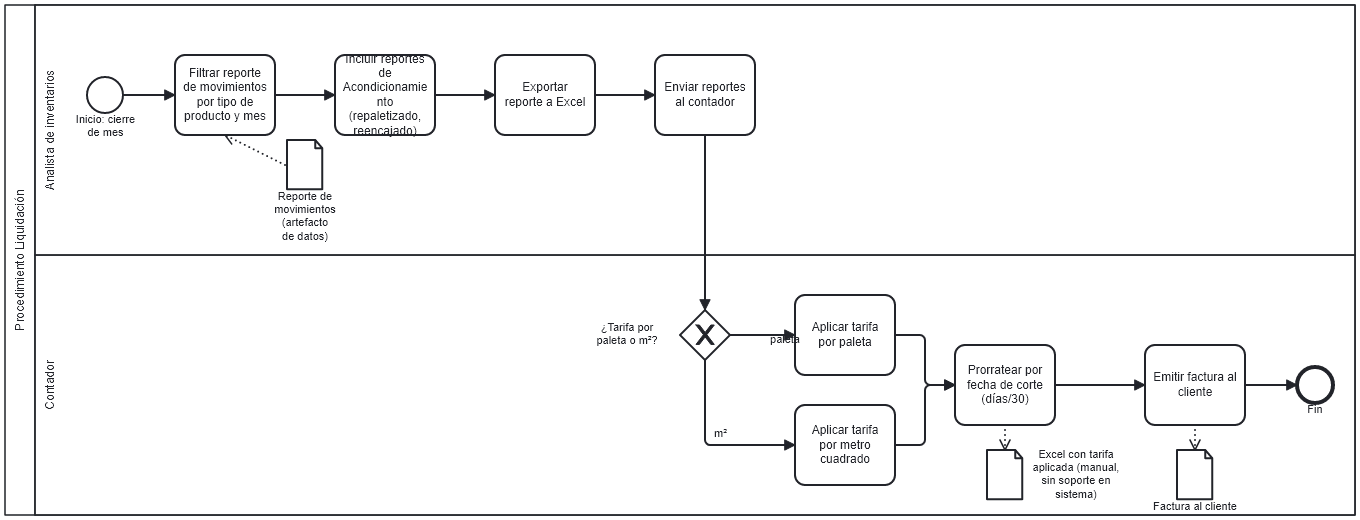
\includegraphics[width=0.9\textwidth]{./imagenes/Facturación.png}
  \caption{Diagrama de Actividades con BPMN - Liquidación mensual in-out y servicios}
\end{figure}

\newpage

% ==========================================
\chapter{Matriz de Indicadores}
% ==========================================
\newpage

\fichaIndicador
  {1. Registro de pedido de ingreso}
  {Exactitud del registro de ingreso}
  {Medir el porcentaje de pedidos de ingreso registrados sin necesidad de modificación posterior}
  {(Pedidos de ingreso aprobados sin observación / Total de pedidos de ingreso del periodo) × 100}
  {IND-REC-01}
  {Supervisor}
  {Analista de inventarios}
  {Por definir}
  {Mensual}

\fichaIndicador
  {2. Verificación y conformidad (Recepción)}
  {Tasa de observación en recepción}
  {Medir la frecuencia de modificaciones por discrepancia entre lo declarado en la guía y lo recibido físicamente}
  {(Pedidos de ingreso con observación / Total de pedidos de ingreso del periodo) × 100}
  {IND-REC-02}
  {Supervisor}
  {Auxiliar de almacén}
  {Por definir}
  {Mensual}

\fichaIndicador
  {3. Registro de pedido de salida}
  {Exactitud del registro de salida}
  {Medir el porcentaje de pedidos de salida registrados conforme a la solicitud del cliente (código, lote y fecha de vencimiento)}
  {(Pedidos de salida aprobados sin observación / Total de pedidos de salida del periodo) × 100}
  {IND-DES-01}
  {Supervisor}
  {Analista de inventarios}
  {Por definir}
  {Mensual}

\fichaIndicador
  {4. Verificación y conformidad (Despacho)}
  {Tasa de observación en despacho}
  {Medir la frecuencia de modificaciones por discrepancia entre el pedido de salida y la mercadería despachada}
  {(Pedidos de salida con observación / Total de pedidos de salida del periodo) × 100}
  {IND-DES-02}
  {Supervisor}
  {Auxiliar de almacén}
  {Por definir}
  {Mensual}

\fichaIndicador
  {5. Transferencia de ubicación}
  {Volumen de transferencias internas}
  {Medir la cantidad de transferencias de ubicación ejecutadas en el periodo, como indicador de reacomodo del almacén}
  {Número total de transferencias ejecutadas en el periodo}
  {IND-ALM-01}
  {Analista de inventarios}
  {Analista de inventarios}
  {Por definir}
  {Mensual}

\fichaIndicador
  {6. Reempaque}
  {Tasa de reempaque sobre recepciones}
  {Medir la proporción de paletas recepcionadas que requieren reempaque por discrepancia con la guía de remisión}
  {(Reempaques ejecutados / Total de paletas recepcionadas en el periodo) × 100}
  {IND-ALM-02}
  {Analista de inventarios}
  {Auxiliar de almacén}
  {Por definir}
  {Mensual}

\fichaIndicador
  {7. Repaletizado}
  {Volumen de repaletizado facturable}
  {Medir la cantidad de paletas repaletizadas por tipo de producto en el periodo, como base de facturación del servicio}
  {Número de paletas repaletizadas por código / tipo de producto en el periodo}
  {IND-ACO-01}
  {Auxiliar de almacén}
  {Auxiliar de almacén}
  {Por definir}
  {Mensual}

\fichaIndicador
  {8. Reencajado}
  {Volumen de reencajado facturable}
  {Medir la cantidad de unidades reencajadas por tipo de producto en el periodo, como base de facturación del servicio}
  {Número de unidades reencajadas por código / tipo de producto en el periodo}
  {IND-ACO-02}
  {Auxiliar de almacén}
  {Auxiliar de almacén}
  {Por definir}
  {Mensual}

\fichaIndicador
  {9. Liquidación mensual in-out y servicios}
  {Oportunidad de facturación}
  {Medir el tiempo transcurrido entre el cierre de mes y la emisión efectiva de la factura al cliente}
  {Fecha de emisión de factura − Fecha de cierre de mes (en días)}
  {IND-FAC-01}
  {Contador}
  {Analista de inventarios}
  {Por definir}
  {Mensual}

\newpage

% ==========================================
\chapter{Documentos Generados}
% ==========================================

% ------------------------------------------
\section*{1. Registro de pedido de ingreso}
% ------------------------------------------
\begin{tabularx}{\textwidth}{>{\raggedright\arraybackslash}X >{\raggedright\arraybackslash}p{0.15\textwidth} >{\raggedright\arraybackslash}p{0.18\textwidth} >{\raggedright\arraybackslash}X}
\toprule
\multirow{2}{*}{\textbf{DOCUMENTO (QUÉ)}} & \multicolumn{3}{c}{\textbf{CUSTODIA}} \\
\cmidrule{2-4}
& \textbf{QUIÉN} & \textbf{DÓNDE} & \textbf{CÓMO} \\
\midrule
Guía de remisión del cliente & Analista de inventarios & Almacén Co Logistic SAC & Recibida por correo, físico o WhatsApp; conservada hasta su engrampado con el pedido de ingreso \\
\midrule
Pedido de ingreso (borrador) & Analista de inventarios & Sistema de almacén & Registro digital previo a firma y aprobación \\
\bottomrule
\end{tabularx}

\vspace{2em}

% ------------------------------------------
\section*{2. Verificación y conformidad (Recepción)}
% ------------------------------------------
\begin{tabularx}{\textwidth}{>{\raggedright\arraybackslash}X >{\raggedright\arraybackslash}p{0.15\textwidth} >{\raggedright\arraybackslash}p{0.18\textwidth} >{\raggedright\arraybackslash}X}
\toprule
\multirow{2}{*}{\textbf{DOCUMENTO (QUÉ)}} & \multicolumn{3}{c}{\textbf{CUSTODIA}} \\
\cmidrule{2-4}
& \textbf{QUIÉN} & \textbf{DÓNDE} & \textbf{CÓMO} \\
\midrule
Pedido de ingreso firmado + guía de remisión & Supervisor / Archivo de almacén & Almacén Co Logistic SAC & Impreso y engrampado físicamente a la guía del cliente; archivo físico \\
\bottomrule
\end{tabularx}

\vspace{2em}

% ------------------------------------------
\section*{3. Registro de pedido de salida}
% ------------------------------------------
\begin{tabularx}{\textwidth}{>{\raggedright\arraybackslash}X >{\raggedright\arraybackslash}p{0.15\textwidth} >{\raggedright\arraybackslash}p{0.18\textwidth} >{\raggedright\arraybackslash}X}
\toprule
\multirow{2}{*}{\textbf{DOCUMENTO (QUÉ)}} & \multicolumn{3}{c}{\textbf{CUSTODIA}} \\
\cmidrule{2-4}
& \textbf{QUIÉN} & \textbf{DÓNDE} & \textbf{CÓMO} \\
\midrule
Guía de remisión del cliente & Analista de inventarios & Almacén Co Logistic SAC & Recibida por correo o físico; conservada hasta su engrampado con el pedido de salida \\
\midrule
Pedido de salida (P.S., borrador) & Analista de inventarios & Sistema de almacén & Registro digital previo a firma y aprobación \\
\bottomrule
\end{tabularx}

\vspace{2em}

% ------------------------------------------
\section*{4. Verificación y conformidad (Despacho)}
% ------------------------------------------
\begin{tabularx}{\textwidth}{>{\raggedright\arraybackslash}X >{\raggedright\arraybackslash}p{0.15\textwidth} >{\raggedright\arraybackslash}p{0.18\textwidth} >{\raggedright\arraybackslash}X}
\toprule
\multirow{2}{*}{\textbf{DOCUMENTO (QUÉ)}} & \multicolumn{3}{c}{\textbf{CUSTODIA}} \\
\cmidrule{2-4}
& \textbf{QUIÉN} & \textbf{DÓNDE} & \textbf{CÓMO} \\
\midrule
Pedido de salida firmado + guía de remisión & Supervisor / Archivo de almacén & Almacén Co Logistic SAC & Impreso y engrampado físicamente a la guía del cliente; archivo físico \\
\bottomrule
\end{tabularx}

\vspace{2em}

% ------------------------------------------
\section*{5. Transferencia de ubicación}
% ------------------------------------------
\begin{tabularx}{\textwidth}{>{\raggedright\arraybackslash}X >{\raggedright\arraybackslash}p{0.15\textwidth} >{\raggedright\arraybackslash}p{0.18\textwidth} >{\raggedright\arraybackslash}X}
\toprule
\multirow{2}{*}{\textbf{DOCUMENTO (QUÉ)}} & \multicolumn{3}{c}{\textbf{CUSTODIA}} \\
\cmidrule{2-4}
& \textbf{QUIÉN} & \textbf{DÓNDE} & \textbf{CÓMO} \\
\midrule
Reporte de movimientos (registro de transferencia) & Analista de inventarios & Sistema de almacén & Generado automáticamente al ejecutar la transferencia; consultable por código, lote o periodo \\
\bottomrule
\end{tabularx}

\vspace{2em}

% ------------------------------------------
\section*{6. Reempaque}
% ------------------------------------------
\begin{tabularx}{\textwidth}{>{\raggedright\arraybackslash}X >{\raggedright\arraybackslash}p{0.15\textwidth} >{\raggedright\arraybackslash}p{0.18\textwidth} >{\raggedright\arraybackslash}X}
\toprule
\multirow{2}{*}{\textbf{DOCUMENTO (QUÉ)}} & \multicolumn{3}{c}{\textbf{CUSTODIA}} \\
\cmidrule{2-4}
& \textbf{QUIÉN} & \textbf{DÓNDE} & \textbf{CÓMO} \\
\midrule
Reporte de movimientos (registro de reempaque) & Analista de inventarios & Sistema de almacén & Generado automáticamente al ejecutar el reempaque; refleja la división de la paleta \\
\bottomrule
\end{tabularx}

\vspace{2em}

% ------------------------------------------
\section*{7. Repaletizado}
% ------------------------------------------
\begin{tabularx}{\textwidth}{>{\raggedright\arraybackslash}X >{\raggedright\arraybackslash}p{0.15\textwidth} >{\raggedright\arraybackslash}p{0.18\textwidth} >{\raggedright\arraybackslash}X}
\toprule
\multirow{2}{*}{\textbf{DOCUMENTO (QUÉ)}} & \multicolumn{3}{c}{\textbf{CUSTODIA}} \\
\cmidrule{2-4}
& \textbf{QUIÉN} & \textbf{DÓNDE} & \textbf{CÓMO} \\
\midrule
Reporte manual de repaletizado & Auxiliar de almacén & Archivo manual (hoja de cálculo) & Elaborado a mano, sin soporte en el sistema; remitido a Facturación \\
\bottomrule
\end{tabularx}

\vspace{2em}

% ------------------------------------------
\section*{8. Reencajado}
% ------------------------------------------
\begin{tabularx}{\textwidth}{>{\raggedright\arraybackslash}X >{\raggedright\arraybackslash}p{0.15\textwidth} >{\raggedright\arraybackslash}p{0.18\textwidth} >{\raggedright\arraybackslash}X}
\toprule
\multirow{2}{*}{\textbf{DOCUMENTO (QUÉ)}} & \multicolumn{3}{c}{\textbf{CUSTODIA}} \\
\cmidrule{2-4}
& \textbf{QUIÉN} & \textbf{DÓNDE} & \textbf{CÓMO} \\
\midrule
Reporte manual de reencajado & Auxiliar de almacén & Archivo manual (hoja de cálculo) & Elaborado a mano, sin soporte en el sistema; remitido a Facturación \\
\bottomrule
\end{tabularx}

\vspace{2em}

% ------------------------------------------
\section*{9. Liquidación mensual in-out y servicios}
% ------------------------------------------
\begin{tabularx}{\textwidth}{>{\raggedright\arraybackslash}X >{\raggedright\arraybackslash}p{0.15\textwidth} >{\raggedright\arraybackslash}p{0.18\textwidth} >{\raggedright\arraybackslash}X}
\toprule
\multirow{2}{*}{\textbf{DOCUMENTO (QUÉ)}} & \multicolumn{3}{c}{\textbf{CUSTODIA}} \\
\cmidrule{2-4}
& \textbf{QUIÉN} & \textbf{DÓNDE} & \textbf{CÓMO} \\
\midrule
Reporte consolidado de movimientos (Excel) & Analista de inventarios & Archivo digital (hoja de cálculo) & Exportado mensualmente del sistema; remitido al contador \\
\midrule
Excel con tarifa aplicada & Contador & Archivo del contador & Elaborado manualmente, sin soporte en el sistema; incluye prorrateo por fecha de corte \\
\midrule
Factura al cliente & Contador & Archivo del contador / SUNAT & Emitida conforme a la normativa de comprobantes de pago electrónicos \\
\bottomrule
\end{tabularx}

\vspace{2em}

% ==========================================
\chapter{Anexos}
% ==========================================
\textbf{ANEXO N° 01:} Transcripción de entrevistas al Analista de Inventarios de Co Logistic SAC (Recepción, Despacho, Almacenamiento, Acondicionamiento, Facturación, Puestos y áreas) \\
\textbf{ANEXO N° 02:} Borrador manuscrito del diagrama de flujo de Recepción y Despacho, elaborado por el Analista de Inventarios \\
\textbf{ANEXO N° 03:} Muestra de Guía de Remisión Electrónica Remitente (Panificadora Bimbo del Perú S.A.) con sello de recepción/despacho de Co Logistic SAC \\
\textbf{ANEXO N° 04:} Diagramas BPMN 2.0 (formato Mermaid .mmd) de los procedimientos documentados

\end{document}
